\documentclass{article}

\usepackage{graphicx}
\usepackage{geometry}
\usepackage{amsmath}
\usepackage{float}

\begin{document}
\noindent
Oliver Evans \\
\today \\

\noindent
\section{Assumptions}
\begin{itemize}
	\item Rope is vertical.
	\item Kelp is horizontal.
	\item Kelp is infinitesimally thin.
	\item Light comes straight down.
	\item Plants are evenly spaced with spacing $\Delta z$.
	\item Each plant absorbs a certain percentage of the light it receives, denoted by $\alpha$.
	\item The lengths of kelp plants in the x direction are normally distributed with mean $\mu$ and standard deviation $\sigma$.
\end{itemize}

That is, the lengths are distributed as
\begin{equation}
	p(l)=\frac{1}{\sqrt{2\pi}\sigma} e^{-\frac{1}{2}\left(\frac{l-\mu}{\sigma}\right)^2}
\end{equation}

\section{Analysis}
Then for the $kth$ plant from the top, at a horizontal position $x$, the expected number of plants shading this spot is 
\begin{align}
	\begin{split}
	N(k,x)&=(k-1)\cdot p(l\geq x) \\
	&=(k-1)\int_x^\infty p(l)\,dl \\
	&=(k-1)\int_x^\infty\frac{1}{\sqrt{2\pi}\sigma} e^{-\frac{1}{2}\left(\frac{l-\mu}{\sigma}\right)^2} \,dl \\
	&=\frac{k-1}{2}\left[1-\mbox{erf}\left(\frac{x-\mu}{\sqrt{2}\sigma}\right)\right] \\
	\end{split}
\end{align}

where \[\mbox{erf}(x)=\frac{2}{\sqrt\pi}\int_0^xe^{-t^2}\,dt\] \\

The irradiance as a function of depth and length is given by
\begin{equation}
	I(z,x)=I_0(1-\alpha)^{N(k,x)}e^{-K_dz}
\end{equation}

\section{Plot}
The following parameters are used in the plot below.
\begin{align*}
	z_{max} &= 10 \\
	x_{max} &= 10 \\
	\alpha &= 0.1 \\
	I_0&=5 \\
	K_d &= 0.1 \\
	\Delta z &= 1
\end{align*}

\vspace{-2em}
\begin{figure}[H]
	\centering
	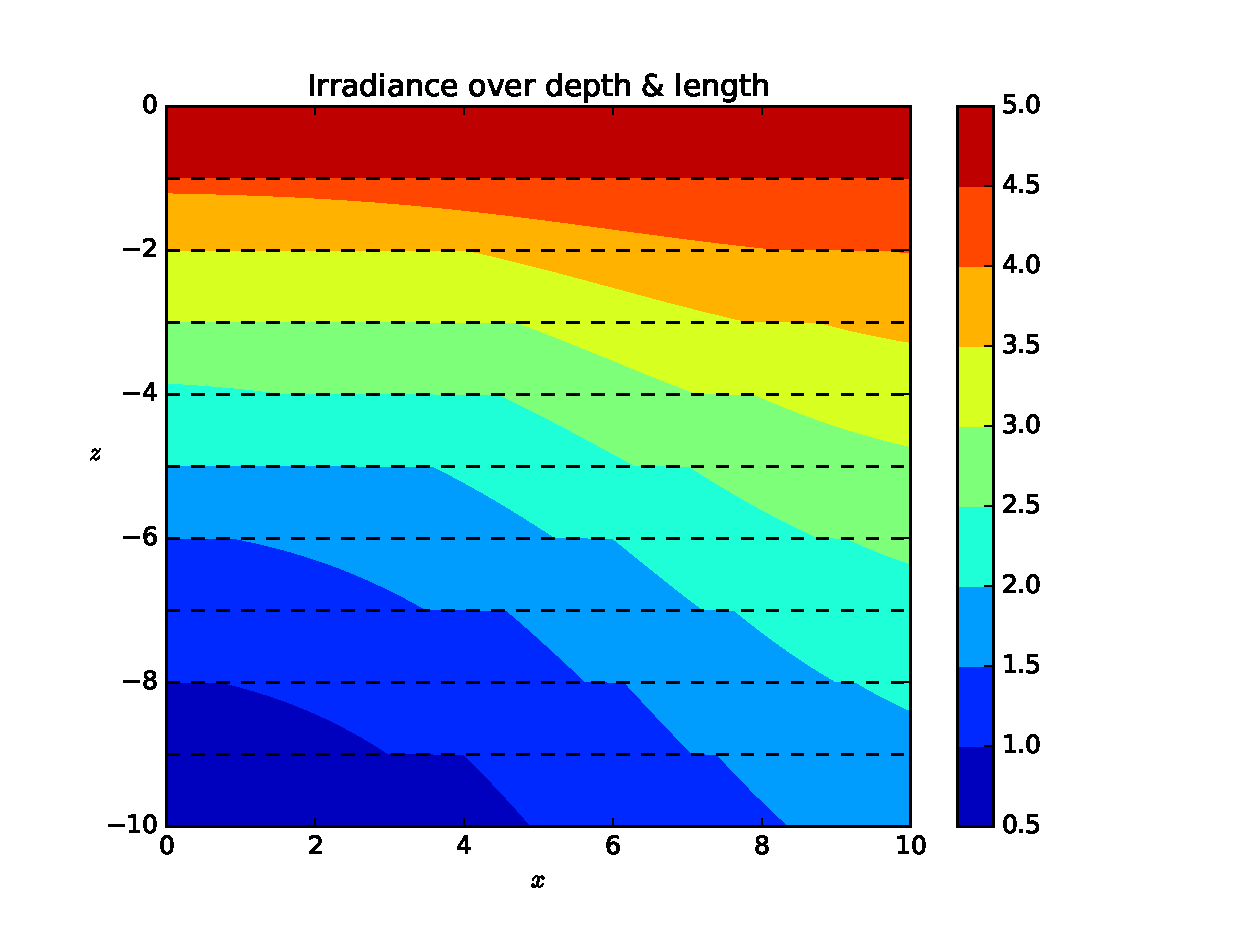
\includegraphics[width=6in]{normal_length.eps}
	\caption{Irradiance as a function of space}
\end{figure}


\end{document}
